%\newpage
\section{Execution}
\label{sec:execution}
\section{Components}
\subsection{Arduino Uno}
The Arduino Uno is a microcontroller board which can be progrmmed with C++ Code to do send and recive different electronic signals.
The arduino board has different analog and digital inputs and outputs which can be connected to electrical cicuits to work with components like sensors, LEDs or diferent logical components.
\subsection{LED}
LED is short for Light Emitting Diode and therefore LED's are a special kind of Diode which emits light if a current is applied.
Diodes are electrical components whose conductivity depends on the applied pooling.
Classical semiconducter diodes are based on the physical properties of a pn-junction as explained in \cite{elektronik-kompendium}.
\subsection{Temperature Sensor DS18B20}
The DS18B20 is a programmable thermometer that can be controlled via a single cable.
Special advantages of the temperature sensor are that it requires only one cable for control besides the ground connection and due to the unique 64-bit serial codes of the sensors it is possible to control multiple sensors with a single cable.
In the range of \SI{-10}{\celsius} to \SI{85}{\celsius}, the temperature sensor has an accuracy of $\pm 0.5$\si{\celsius} and can be used in a temperature range from \SI{-55}{\celsius} to \SI{125}{\celsius}.
With the help of a prasitic power mode it is even possible to operate the temperature sensor with only 2 connections (GND and DQ) whereby the power supply is then also provided via the signal connection. In our case, however, we used 3 cables for operation.
Because the temperature sensor is connected to a 3-state port for its input signal, a pull-up resistor is used on the control line.

\subsection{Experiment}
The different Thermometers from the Arduino Circuits are connected to a handheld lab thermometer in a way that all thermometer tips align.
For the expirement a watertank with a heating/cooling plate and a pump to mix up the watercolumn is brought to a temperature of \SI{3}{\celsius} while the surronding air temperature is at \SI{25}{\celsius}.
To calibrate the sensors, all connected sensors are immersed in the water bath at the same time.
After a short time the temperature of the water bath is changed and increased to \SI{20}{\celsius}.
Each difference of \SI{1}{\kelvin} is noted with the corresponding timestamp.

\subsection{Arduino Wiring}
The arduino wiring is shown in Figures \ref{fig:wiring1} and \ref{fig:wiring2}.
\begin{figure}
    \centering 
    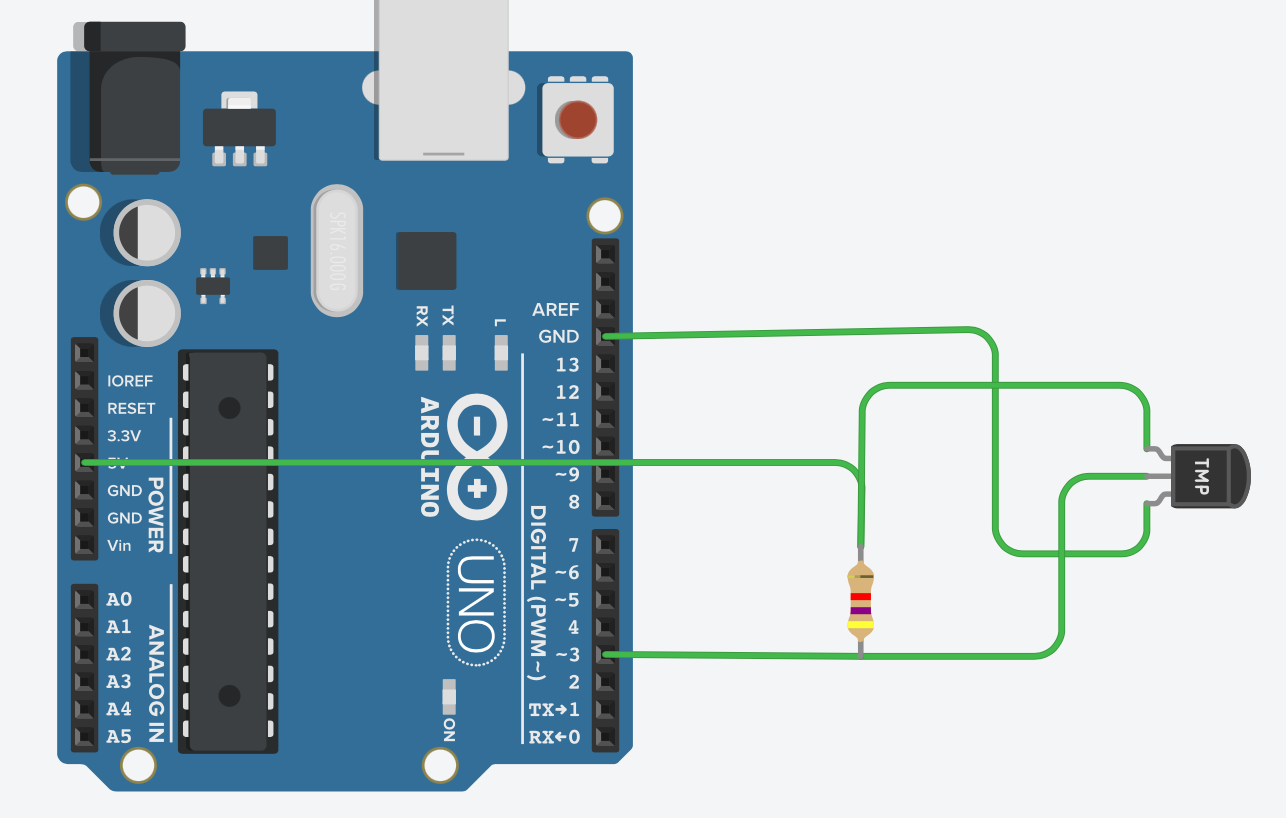
\includegraphics[width = 0.8\textwidth]{bilder/wiring_1.png}
    \label{fig:wiring1}
\end{figure}
\begin{figure}
    \centering 
    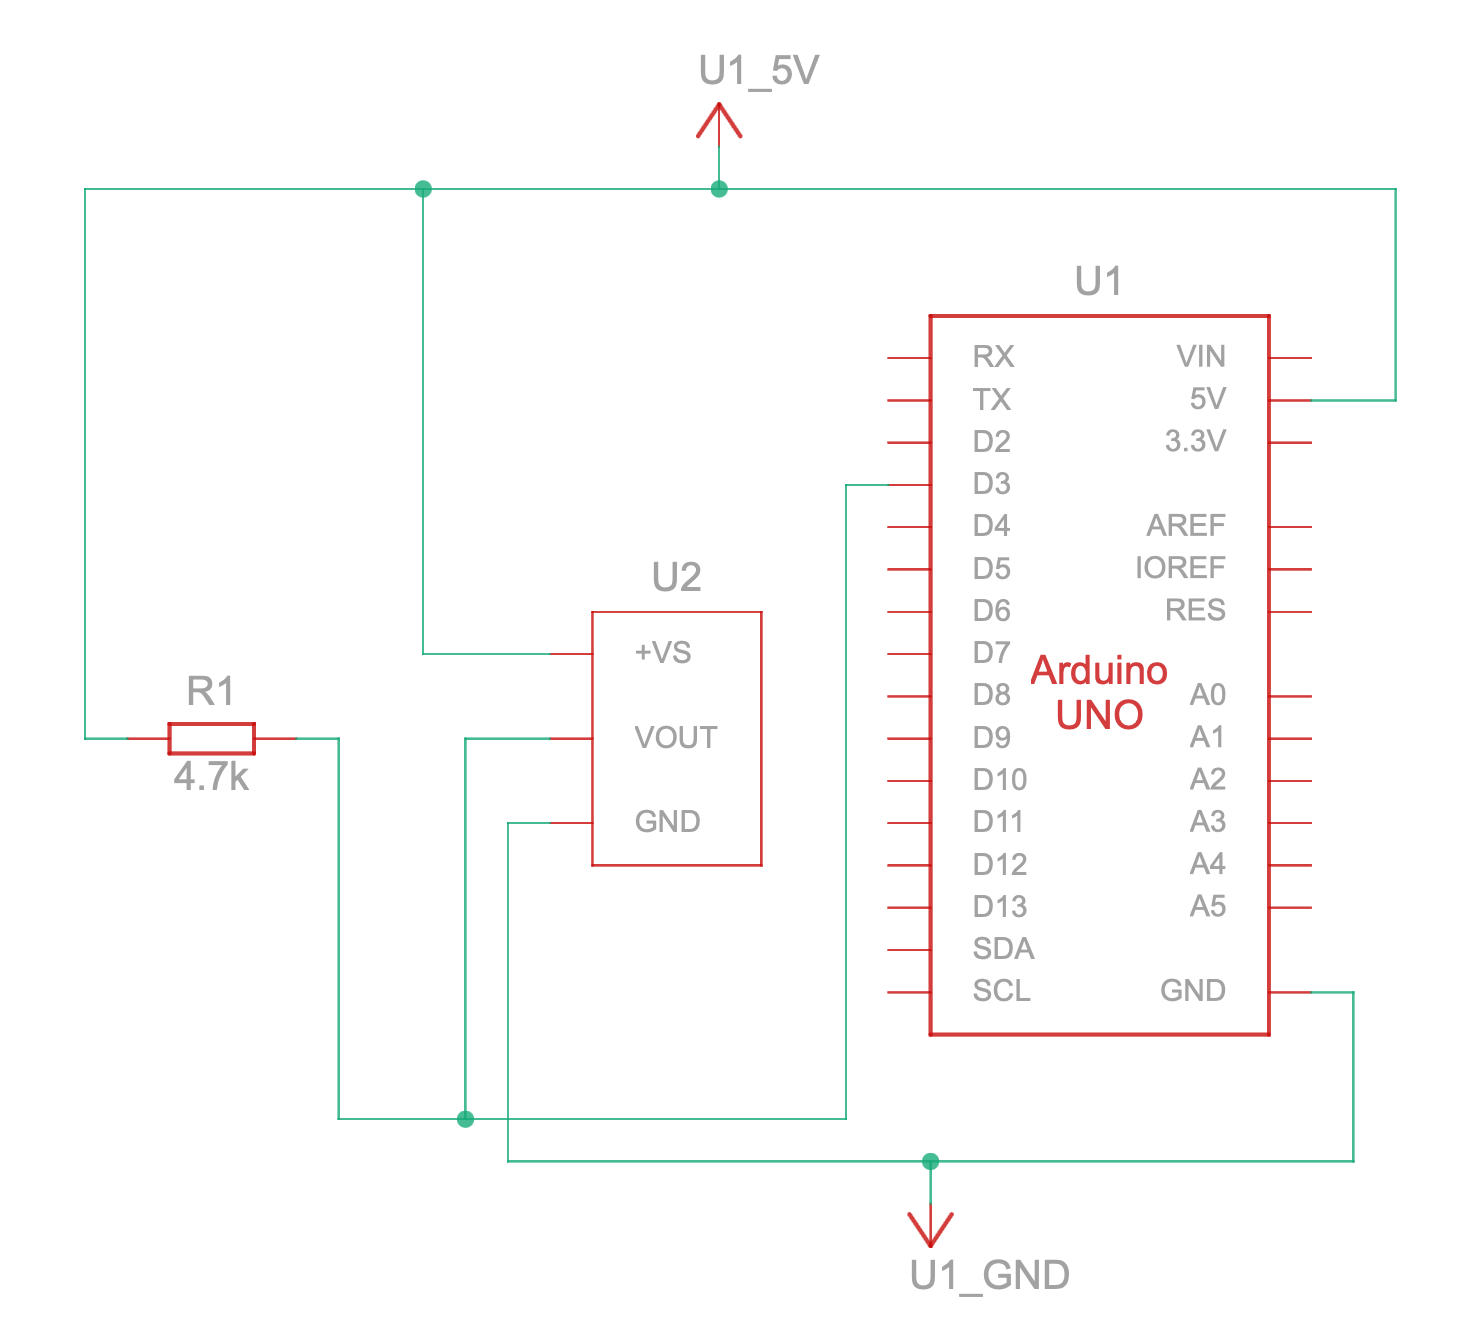
\includegraphics[width = 0.8\textwidth]{bilder/wiring_2.png}
    \label{fig:wiring2}
\end{figure}
\subsection{Arduino Coding}
To setup the arduino first of all the void function setup() is programmed.
In the setup the Serial output is initialized with a baud rate of 9600.
If the RealTimeClock (rtc) is not running a error message is printed and the rtc will be started.
For the first time running the code the internal clock is initialized with the local Computer time.
Next up the SD card is checked and of its not found an error message is prompted.
The different digital pins are put to the output mode to deliver information to the temperature sensor.
At last the header for the data is saved in the SD card LOG file.

For the measurements a routine is defined in the function loop() for the arduino.

First two arrays are initialized for the scratchpad data and the rom code.
Then the OneWire bus is reset and the Rrom code is read to save the registration number or ID of the sensor.
Afterwards the OneWire test is reset again to save the temperature reading.
The temperature data is converted from binary to decimal and then all readings are saved on the SD card.
At the end a delay of 1000 milliseconds assures that the data is read every second.
\subsection{Adjusting for Average meas}
Before the void setup():
\begin{lstlisting}
int cnt = 0;
float avg = 0;
\end{lstlisting}
In the void loop():
\begin{lstlisting}
if (cnt < 9){
    avg = avg+tempCelsius;
  }
else{
    save_data_point(time_now,registration_number,tempCelsius,avg/10);
    cnt = 0;
  }
delay(1000);
\end{lstlisting}
In the save\_data\_point function:

\begin{lstlisting}
void save_data_point(String time,String reg,float spot,float avg){
  printOutput(time);
  printOutput(", ");
  printOutput(String(millis()));
  printOutput(", ");
  printOutput(reg);
  printOutput(", ");
  printOutput(String(spot));
  printOutput(", ");
  printOutputln(avg);
}
\end{lstlisting}

\subsection{Status LED}
LED with different shades of blue,red and purple depending on the temperature.
\begin{lstlisting}
void LED(int signal){
    if (signal < -55){
        digitalWrite(5,255);
        digitalWrite(6,0);
      }
      else if(signal > 125){
      digitalWrite(6,255);
        digitalWrite(5,0);
      }
      else if (signal > -55 && signal < 125){
        int brightness = ((signal + 55. )/180.)*255;
        analogWrite(5,255 - brightness);
        analogWrite(6,brightness);
      }
}
\end{lstlisting}